\subsection{Прямий метод}

Нагадаємо попередню лекцію: задано рівняння
\begin{equation}
    \label{eq:2.1.1}
    A u = f,
\end{equation}
з пераметром $f \in W_2^{-1}$. Нагадаємо також, що такі умови на праву частину означають, що розв'язок $u \in W_2^1$.

\begin{example}
    Розглянемо рівняння
    \begin{equation}
        \label{eq:2.1.2}
        -(ku')' - pu' + qu = f, \quad a < x < b,
    \end{equation}
    з крайовими умовами
    \begin{equation}
        \label{eq:2.1.3}
        -ku' + \alpha_1 u = \mu_1, \quad x = a,
    \end{equation}
    і
    \begin{equation}
        \label{eq:2.1.4}
        ku' + \alpha_2 u = \mu_2, \quad x = b.
    \end{equation}
\end{example}
\begin{solution}
    Запишемо
    \begin{equation*}
        (A u, v) = (f, v).
    \end{equation*}

    У явному вигляді маємо
    \begin{equation}
        \label{eq:2.1.5}
        \int_a^b (k u' v' - p u' v + q u v) \diff x + \alpha_1 u(a) v(a) + \alpha_2 u(b) v(b) - \mu_1 v(a) - \mu_2 v(b) = \int_a^b f v \diff x.
    \end{equation}
    
    Тут ми скористалися формулою інтегрування за частинами:
    \begin{equation*}
        \int_a^b -(k u')' \diff x = - \left. k u' v \right|_a^b + \int_a^b k u' v' \diff x,
    \end{equation*}
    звідки (а саме з $ku'v|_{x=a}$ і $ku'v|_{x=b}$) і виникли доданки з $\alpha_{1,2}$ та $\mu_{1,2}$.
\end{solution}

\subsection{Метод колокацій}

Розглянемо рівняння
\begin{equation}
    \label{eq:2.5.1}
    A u = f,
\end{equation}
де $A: E \to F$, замінюємо на рівняння
\begin{equation}
    \label{eq:2.5.2}
    P_n(Au_n) = P_n f,
\end{equation}
або на
\begin{equation}
    \label{eq:2.5.3}
    P_n(Au_n - f) = 0.
\end{equation}

Координатну систему візьмемо $\{\phi_i\} \in D(A) \subseteq E$, а проекційну --- $\{\psi_i\}\in F^\star$. Тоді можемо \eqref{eq:2.5.3} переписати у вигляді \[\psi_j(Au_n - f) = 0,\] або \[\psi_j Au_n = \psi_j f.\]

Шукачи розв'язок у вигляді \[u_n = \sum_{i = 1}^n c_i \phi_i,\] матимемо \[ \psi_j \left( A \left( \sum_{i = 1}^n c_i \phi_i \right) \right) = \psi_j f, \] або ж, враховучи лінійність,
\begin{equation}
    \label{eq:2.5.4}
    \sum_{i = 1}^n c_i \psi_j \left( A \phi_i \right) = \psi_j f, \quad j = \overline{1,n}.
\end{equation}

Матриця системи вище має вигляд
\begin{equation}
    \label{eq:2.5.5}
    D = \begin{pmatrix}
        \psi_1(A\phi_1) & \psi_1(A\phi_2) & \cdots & \psi_1(A\phi_n) \\
        \psi_2(A\phi_1) & \psi_2(A\phi_2) & \cdots & \psi_2(A\phi_n) \\
        \vdots & \vdots & \ddots & \vdots \\
        \psi_n(A\phi_1) & \psi_n(A\phi_2) & \cdots & \psi_n(A\phi_n)
    \end{pmatrix}
\end{equation}

Якщо взяти у якості $\{\psi_j\}$ систему функцій Чебишова, то отримаємо $|D| \ne 0$.

\begin{example}
    Нехай $F = C([a,b])$, і візьмемо $\psi_j(f) = f(x_j)$, де $x_j$ --- множина попарно різних вузлів на $[a,b]$.
\end{example}

\begin{example}
    Розглянемо рівняння \[-(ku')' - pu' + qu = f, \quad a < x < b,\] з крайовими умовами \[u(0) = u(1) = 0.\]
\end{example}

\begin{solution}
    Візьмемо \[\omega_n = \{x_j = j h, h = 1 / n\},\] тоді шукачи розв'язок у вигляді \[u_n = \sum_{i = 1}^n c_i \phi_i,\] отримаємо систему
    \begin{equation}
        \label{eq:2.5.6}
        \sum_{i = 1}^n c_i ((-k(x_j)\phi_i'(x_j))-p(x_j)\phi_i'(x_j)+q(x_j)\phi_i(x_j)) = f(x_j), \quad j = \overline{1,n}.
    \end{equation}
\end{solution}

\begin{remark}
    На практиці метод колокацій збігається ще повільніше ніж метод Бубнова-Гальоркіна, але він зручний в випадках, коли розв'язки мають різні градієнти:
    \begin{figure}[H]
        \centering
        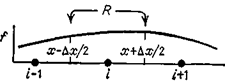
\includegraphics[width=.5\textwidth]{{img/02/04}.png}
        \caption{Покращуємо точність за рахунок скупчення точок $x_j$ у регіонах де розв'язок має великий градієнт.}
    \end{figure}
\end{remark}

\begin{example}
    Нехай задано неоднорідну задачу
    \begin{equation}
        \label{eq:2.5.7}
        A u \equiv (-ku')' - pu' + qu = f
    \end{equation}
    з умовами
    \begin{equation}
        \label{eq:2.5.8}
        u(0) = C, \quad u(1) = D.
    \end{equation}
\end{example}
\begin{solution}
    Тоді розв'язок шукаємо у вигляді
    \begin{equation}
        \label{eq:2.5.9}
        u = v + \phi_0,
    \end{equation}
    де $\phi_0$ --- відома функція що задовольняє неоднорідним крайовим умовами, наприклад $\phi_0(x) = C + x (D - C)$. Тоді матимето \[A v + A \phi_0 = f,\] або ж
    \begin{equation}
        \label{eq:2.5.10}
        A v = f - A \phi_0 = f_1,
    \end{equation}
    з умовами
    \begin{equation}
        \label{eq:2.5.11}
        v(0) = v(1) = 0.
    \end{equation}
    
    За розв'язком цього рівняння відновлюється розв'язок початкового за формулою $u_n = v_n + \phi_0$.
\end{solution}

\section{Варіаційні методи розв'язування крайових задач}

Розглянемо рівняння
\begin{equation}
    \label{eq:3.1}
    A u = f,
\end{equation}
де $A: E \to F$, $E, F$ --- пара гільбертових просторів. Припустимо також, що існує і єдиний розв'язок задачі \eqref{eq:3.1}. \medskip

Ідея варіаційних методів полягає у тому, що ми будемо зводити задачу \eqref{eq:3.1} до знаходження мінімуму деякого функціоналу, що відповідає цій задачі, а саме $\Phi(u): E \to \RR$,
\begin{equation}
    \label{eq:3.2}
    \inf_{u \in E} \Phi(u) = \Phi_0.
\end{equation}

\subsection{Загальні положення задачі мінімізації функціоналів}

Нехай $G(u, v)$ --- білінійна симетрична функція (функціонал) у дійсному гільбертовому просторі.

\begin{definition}
    Функціонал $G$ називається \textit{додатним}, якщо $G(u, u) > 0$, $\forall u \in D(G) \setminus \{0\}$.
\end{definition}

\begin{definition}
    Функціонал $G$ називається \textit{додатно визначеним}, якщо
    \begin{equation}
        \label{eq:3.3}
        G(u, u) > \mu \|u\|^2, \quad \forall u \in D(G) \setminus \{0\},
    \end{equation}
    де $\mu > 0$.
\end{definition}

Визначимо функціонал $\Phi$ наступним чином:
\begin{equation}
    \label{eq:3.4}
    \Phi(u) = G(u,u) - 2 \ell(u) + C,
\end{equation}
де $\ell(u)$ --- лінійний функціонал з не вужчою областю визначення ніж $G$, тобто $D(G) \subseteq D(\ell)$, а $C$ --- довільна (можливо навіть від'ємна) константа.

\begin{lemma}
    Нехай $G(u, u)$ --- додатно визначений, а $\ell(u)$ --- обмежений, тоді $\Phi(u)$ --- обмежений знизу.
\end{lemma}
\begin{remark}
    Тут \textit{обмеженість} $\ell$ розуміється у тому сенсі, що $\exists a > 0$: $\|\ell(u)\| \le a \|u\|$.
\end{remark}
\begin{proof}
    Безпосередньо з \eqref{eq:3.4} і \eqref{eq:3.3} маємо
    \begin{equation}
        \label{eq:3.5}
        \|\Phi(u)\| \ge \mu \|u\|^2 - 2 a \|u\| + C,
    \end{equation}
    Роблячи заміну змінної $x = \|u\|$ і перепозначаючи праву частину за $f(x)$ отримаємо
    \begin{equation*}
        f(x) = \mu x^2 - 2 a x + C,
    \end{equation*}
    а це парабола з гілками вгору, у якої існує мінімум, який досягається в $x_0 = \frac{a}{\mu}$, і дорівнює $C - \frac{a^2}{\mu}$.
\end{proof}

\begin{corollary}
    $\exists u^\star$: $\inf_{u \in D(G)} \Phi(u) = \Phi_0 = \Phi(u^\star)$.
\end{corollary}
\begin{proof}
    Див. книгу Ляшка, Макарова і Скоробагатька, або ж Ліонса.    
\end{proof}

\begin{theorem}
    Нехай
    \item \begin{equation}
        \exists u^\star \in D(G),
        \label{eq:3.1.6}
    \end{equation}
    тоді виконуються наступні умови
    \begin{enumerate}
        \item \begin{equation}
            \label{eq:3.1.7}
            G(u^\star, v) = \ell(v), \quad \forall v \in D(G)
        \end{equation}
        \item \begin{equation}
            \label{eq:3.1.8}
            \Phi(u^\star + v) = \Phi(u^\star) + G(v, v).
        \end{equation}
    \end{enumerate}
\end{theorem}
\begin{proof}
    \begin{equation}
        \label{eq:3.1.9}
        \begin{aligned}
            \Phi(u^\star + v) 
            &= G(u^\star + v, u^\star + v) - 2 \ell(u^\star + v) + C = \\
            &= G(u^\star, u^\star) + G(v, v) + G(u^\star, v) - 2 \ell(u^\star) - 2 \ell(v) + C = \\
            &= \Phi(u^\star) + \Big( 2 (G(u^\star, v) - \ell(v)) + G(v, v) \Big) \ge  \\
            &\ge \Phi(u^\star).
        \end{aligned}
    \end{equation}
    Тоді
    \begin{equation}
        \label{eq:3.1.10}
        2 (G(u^\star, v) - \ell(v)) + G(v, v) \ge 0.
    \end{equation}
    Тоді це виконується і для $v := t v$, тобто
    \begin{equation}
        \label{eq:3.1.11}
        2 t (G(u^\star, v) - \ell(v)) + t^2 G(v, v) \ge 0,
    \end{equation}
    причому можемо взяти $t$ таким, аби перший доданок переважав другий за модулем, і був від'ємний за знаком. Тоді нерівність можлива якщо і тільки якщо
    \begin{equation}
        \label{eq:3.1.12}
        G(u^\star, v) = \ell(v),
    \end{equation}
    а це ніщо янше як \eqref{eq:3.1.7}. Підставляючи \eqref{eq:3.1.12} в \eqref{eq:3.1.9} отримуємо \eqref{eq:3.1.8}
\end{proof}

\begin{definition}
    Послідовність $\{u_n\}$ називається \textit{мінімізуючою} для $\Phi$, якщо
    \begin{equation*}
        \lim_{n \to \infty} \Phi(u_n) = \Phi(u^\star) = \inf \Phi(u) = \Phi_0.
    \end{equation*}
\end{definition}

\begin{theorem}
    Нехай $\{u_n\}$ мінімізуюча для $\Phi$, тоді вона фундаментальна і збігається до $u^\star$ у розумінні відстані
    \begin{equation}
        \label{eq:3.1.14}
        \rho_G(u, v) = \sqrt{G(u - v, u - v)}.
    \end{equation}
\end{theorem}
\begin{proof}
    Наступні дві нерівності справджуються (як наслідок з визначення інфімума) для достатньо великого $N$ і $n,m>N$:
    \begin{align*}
        \Phi(u_n) &\le \Phi_0 + \epsilon, \\
        \Phi(u_m) &\le \Phi_0 + \epsilon.
    \end{align*}
    
    У сумі маємо
    \begin{equation*}
        \begin{aligned}
            \Phi(u_n) + \Phi(u_m) 
            &\le 2 \Phi_0 + 2 \epsilon \le \\
            &\le 2 \Phi \left( \frac{u_n + u_m}{2} \right) + 2 \epsilon.
        \end{aligned}
    \end{equation*}
    
    Тоді шляхом нескладних арифметичних перетворень маємо
    \begin{equation}
        \label{eq:3.1.15}
        2 \epsilon \ge \Phi(u_n) + \Phi(u_m) - 2 \Phi \left( \frac{u_n + u_m}{2} \right) = \frac{1}{2} G(u_m - u_n, u_m - u_n).
    \end{equation}
    
    Підставляючи сюди \eqref{eq:3.1.14} маємо
    \stepcounter{equation}
    \begin{equation}
        \label{eq:3.1.16}
        \rho^2(u_n, u_m) \le 4 \epsilon,
    \end{equation}
    тобто
    \begin{equation*}
        \rho(u_n, u_m) \le 2 \sqrt{\epsilon},
    \end{equation*}
    що говорить про фундаментальність $\{u_n\}$.
\end{proof}
    
\begin{exercise}
    Переконатися в істинності рівності в \eqref{eq:3.1.15}.
\end{exercise}
\begin{solution}
    Нескладні арифметичні перетворення:
    \begin{equation*}
        \begin{aligned}
            & \Phi(u_n) + \Phi(u_m) - 2 \Phi \left( \frac{u_n + u_m}{2} \right) = \\
            &\quad = G(u_n, u_n) - 2 \ell(u_n) + C + G(u_m, u_m) - 2 \ell(u_m) + C - \\
            &\qquad - 2 \left( G \left( \frac{u_n + u_m}{2}, \frac{u_n + u_m}{2} \right) - 2 \ell \left(\frac{u_n + u_m}{2} \right) + C \right) = \\
            &\quad = G(u_n, u_n) + G(u_m, u_m) - 2 G \left( \frac{u_n + u_m}{2}, \frac{u_n + u_m}{2} \right) - \\
            &\qquad - 2 \left( \ell(u_n) + \ell(u_m) - 2\ell\left(\frac{u_n + u_m}{2} \right) \right).
        \end{aligned}
    \end{equation*}
    Другий доданок скорочується за лінійністю $\ell$, а для першого можемо записати:
    \begin{equation*}
        \begin{aligned}
            & G(u_n, u_n) + G(u_m, u_m) - 2 G \left( \frac{u_n + u_m}{2}, \frac{u_n + u_m}{2} \right) = \\
            &\quad = \frac{1}{2} G(u_n, u_n) + \frac{1}{2} G(u_m, u_m) - G(u_n, u_m) = \\
            &\quad = \frac{1}{2} G(u_m - u_n, u_m - u_n),
        \end{aligned}
    \end{equation*}
    що і показує істинність \eqref{eq:3.1.15}.
\end{solution}

\subsubsection{Процес Рітца побудови мінімізаційної послідовності}

\begin{enumerate}
    \item Вибираємо повну лінійно незалежну систему функцій $\{\phi_i\} \in D(G)$.
    
    \item Будуємо простори $H_n = \mathcal{L}(\phi_1,\ldots,\phi_n)$, тоді 
    \begin{equation}
        \label{eq:3.1.17}
        u_n = \sum_{i = 1}^n c_i \phi_i.
    \end{equation}
    
    \item Будемо шукати розв'язок задачі
    \begin{equation}
        \label{eq:3.1.18}
        \inf_{u \in H_n} \Phi(u) = \Phi(u_n).
    \end{equation}
    
    Тоді з \eqref{eq:3.1.7} маємо
    \begin{equation}
        \label{eq:3.1.19}
        G(u_n,v)=\ell(v), \quad \forall v \in H_n.
    \end{equation}
    
    Підставляючи сюди $u_n$ з \eqref{eq:3.1.17} будемо мати
    \begin{equation}
        \label{eq:3.1.20}
        \sum_{i = 1}^n c_i G(\phi_i, v) = \ell(v), \quad \forall v \in H_n,
    \end{equation}
    або ж
    \begin{equation}
        \label{eq:3.1.21}
        \sum_{i = 1}^n c_i G(\phi_i, \phi_j) = \ell(\phi_j), \quad j = \overline{1,n},
    \end{equation}
    отримали систему систему лінійних рівнянь з матрицею Грама на коефіцієнти $c_i$. Якщо система лінійно незалежна то розв'язок існує і єдиний.
\end{enumerate}
